% vim: set ft=tex tabstop=4 shiftwidth=4 noexpandtab:

% header %{{{1

% opening %{{{2

\documentclass[tikz, border=1mm]{standalone}

% packages and libraries %{{{2

% ---- not necessary since the documentclass[tikz ...] requires it automatically
% \usepackage{tikz}

\usepackage{../../include/latex/custom}

\usetikzlibrary{calc,intersections,angles,quotes,shapes.geometric,arrows.meta,decorations.markings}

\usepackage{tkz-euclide}

% colors %{{{2

\definecolor{goldenbrown}{HTML}{5b3c11}

% style %{{{2

\tikzset{
	% ------- every something
	every picture/.style={
		scale=1.0,
	},
	every coordinate/.style={
		fill=black, circle, inner sep=1pt,
	},
	every path/.style={
		line width=0.3pt,
	},
	every node/.style={
		font=\normalsize,
	},
	every angle/.style={
	},
	every pic/.style={
		% ---- does not worl
		%draw,
		%-{Straight Barb[length=1.2mm]},
	},
	% ------- custom
	vector/.style={
		-{Straight Barb[length=1.2mm]},
		%thick,
	},
	mid arrow/.style={
		postaction={
			decorate,
			decoration={
				markings,
				mark=at position #1 with {
					\arrow{Straight Barb[length=1.2mm]}
				}
			}
		}
	},
	mid arrow/.default=0.5,
	construction/.style={
		line width=0.1pt,
		dashed,
	},
	dimension/.style={
		line width=0.2pt,
		<->,
		goldenbrown,
	},
	dimension extension/.style={
		line width=0.2pt,
		dashed,
		goldenbrown,
	},
}

% document %{{{1

% opening %{{{2

\begin{document}
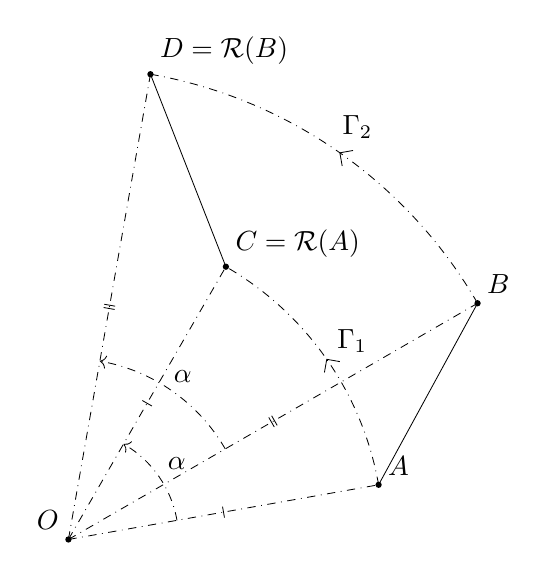
\begin{tikzpicture}[scale=1.0]

% parameters %{{{2

	 \tikzmath{
		\radius1 = 4;
		\radius2 = 6;
		\angrot = 50;
		\ang1 = 10;
		\ang2 = 30;
		\endang1 = \ang1 + \angrot;
		\meanang1 = (\ang1 + \endang1)/2;
		\endang2 = \ang2 + \angrot;
		\meanang2 = (\ang2 + \endang2)/2;
	 }

% coordinates %{{{2

	\coordinate (O) at (0,0);

	\coordinate (A) at (\ang1:\radius1);
	\coordinate (rA) at (\endang1:\radius1);

	\coordinate (B) at (\ang2:\radius2);
	\coordinate (rB) at (\endang2:\radius2);

% points, dots, vertices %{{{2

	\fill (O) circle (0.4mm);
	\fill (A) circle (0.4mm);
	\fill (rA) circle (0.4mm);
	\fill (B) circle (0.4mm);
	\fill (rB) circle (0.4mm);

% segments, sides %{{{2

	\draw (A) -- (B);
	\draw (rA) -- (rB);

	\draw[dashdotted] (O) -- (A);
	\draw[dashdotted] (O) -- (rA);

	\draw[dashdotted] (O) -- (B);
	\draw[dashdotted] (O) -- (rB);

% circles %{{{2

% circular arcs %{{{3

	\draw[mid arrow, dashdotted] (A) arc (\ang1:\endang1:\radius1);
	\draw[mid arrow, dashdotted] (B) arc (\ang2:\endang2:\radius2);

% points, dots, vertices labels %{{{2

	\node[above left] at (O) {$O$};

	\node[above right] at (A) {$A$};
	\node[above right] at (rA) {$C = \mathcal{R}(A)$};

	\node[above right] at (B) {$B$};
	\node[above right] at (rB) {$D = \mathcal{R}(B)$};

% segments, sides labels %{{{2

	%\node[below right] at ($ (O)!0.7!(A) $) {$r$};
	%\node[left] at ($ (O)!0.7!(rA) $) {$r$};

% segments, sides marks %{{{2

	\tkzMarkSegments[mark=|, size=2pt](O,A)
	\tkzMarkSegments[mark=|, size=2pt](O,rA)

	\tkzMarkSegments[mark=||, size=2pt](O,B)
	\tkzMarkSegments[mark=||, size=2pt](O,rB)

% circular arcs labels %{{{2

	\node at (\meanang1:\radius1+0.4) {$\Gamma_1$};
	\node at (\meanang2:\radius2+0.4) {$\Gamma_2$};

% angles labels %{{{2

	\pic[draw, ->, dashdotted, "$\alpha$", angle radius=1.4cm, angle eccentricity=1.2]
	{angle = A--O--rA};

	\pic[draw, ->, dashdotted, "$\alpha$", angle radius=2.3cm, angle eccentricity=1.1]
	{angle = B--O--rB};

% closing %{{{2

\end{tikzpicture}
\end{document}
